\chapter{Calor e isolamento}\label{ch:g5:heat-and-insulation}

Por que o escorregador de metal parece gelado e o banco de madeira ao
lado dele não parece? Esse mistério nos persegue desde o primeiro ano
deste livro. Hoje ele cai --- junto com os segredos da garrafa
térmica, da janela dupla e do pardal todo inflado no inverno. A chave
é parar de perguntar como as coisas \emph{parecem} e começar a seguir
por onde o \omterm{def:g5:heat-and-insulation:heat}{calor} \emph{flui}.

\section{O calor está em trânsito}

\begin{definition}[Calor]\label{def:g5:heat-and-insulation:heat}
\emph{Calor}\index{calor} é \omterm{def:g5:everyday-energy:energy}{energia} em trânsito de um corpo mais
quente para um mais frio. A sopa passa calor para a colher, o
aquecedor passa para a sala, a sua mão passa para uma bola de neve. O
calor não é um material escondido dentro das coisas quentes --- ele é
um \emph{fluxo}, e sempre tem um sentido.
\end{definition}

\begin{proposition}[O calor flui ladeira abaixo]\label{prop:g5:heat-and-insulation:downhill}
Sozinho, o \omterm{def:g5:heat-and-insulation:heat}{calor} sempre flui do corpo mais quente para o mais frio
--- nunca ao contrário. O fluxo corre enquanto as duas \omterm{def:g3:temperature-thermometers:temperature}{temperaturas}
forem diferentes e vai morrendo conforme elas se encontram: deixados
juntos por tempo suficiente, vizinhos quente e frio acabam numa mesma
\omterm{def:g3:temperature-thermometers:temperature}{temperatura}.
\end{proposition}

\begin{example}[Lendo o sentido]\label{ex:g5:heat-and-insulation:direction}
A colherinha no chá esquenta: o \omterm{def:g5:heat-and-insulation:heat}{calor} fluiu do chá $\to$ para a
colher. A limonada com gelo esfria --- cuidado! Não entrou nada
chamado ``frio'': o \omterm{def:g5:heat-and-insulation:heat}{calor} fluiu \emph{da limonada para o gelo},
derretendo-o. O frio não é um fluxo; é só o nome que damos ao lado
perdedor. Todos os livros de física dizem ``a bebida perde \omterm{def:g5:heat-and-insulation:heat}{calor}'',
nunca ``a bebida ganha frio''.
\end{example}

\begin{omfigure}
\begin{tikzpicture}[scale=0.85]
  \draw[thick] (0.6,0.4) rectangle (3.0,1.9);
  \node[font=\small] at (1.8,1.15) {sopa quente};
  \draw[thick] (7.8,0.4) rectangle (10.2,1.9);
  \node[font=\small] at (9.0,1.15) {ar fresco};
  \draw[-Stealth, line width=3pt, omThm] (3.3,1.15) -- (7.5,1.15);
  \node[above, font=\small, omThm] at (5.4,1.4)
    {o calor flui do quente $\to$ para o frio};
  \node[below, font=\small] at (5.4,0.0)
    {e só para quando as duas temperaturas se encontram};
\end{tikzpicture}

{\small Uma regra só para toda cozinha e todo inverno: o \omterm{def:g5:heat-and-insulation:heat}{calor} corre
ladeira abaixo, do mais quente para o mais frio, até a ladeira
acabar.}
\end{omfigure}

\section{Pistas rápidas e pistas lentas}

\begin{definition}[Condutores e isolantes de calor]\label{def:g5:heat-and-insulation:conductors}
Os materiais diferem muitíssimo na rapidez com que deixam o \omterm{def:g5:heat-and-insulation:heat}{calor}
fluir por eles. Um \emph{condutor de calor}\index{condutor de calor}
é uma pista rápida --- os metais acima de todos. Um \emph{isolante
térmico}\index{isolante térmico} é uma pista lenta: madeira, lã,
plástico, penas --- e o campeão, o \emph{\omterm{def:g2:air-around-us:air}{ar} parado}, preso de modo que
não possa rodopiar. (As palavras foram tomadas de propósito dos
\omterm{def:g4:conductors-insulators:conductor}{condutores} e \omterm{def:g4:conductors-insulators:insulator}{isolantes} da eletricidade; as duas propriedades andam
juntas com frequência, mas nem sempre.)
\end{definition}

\begin{omfigure}
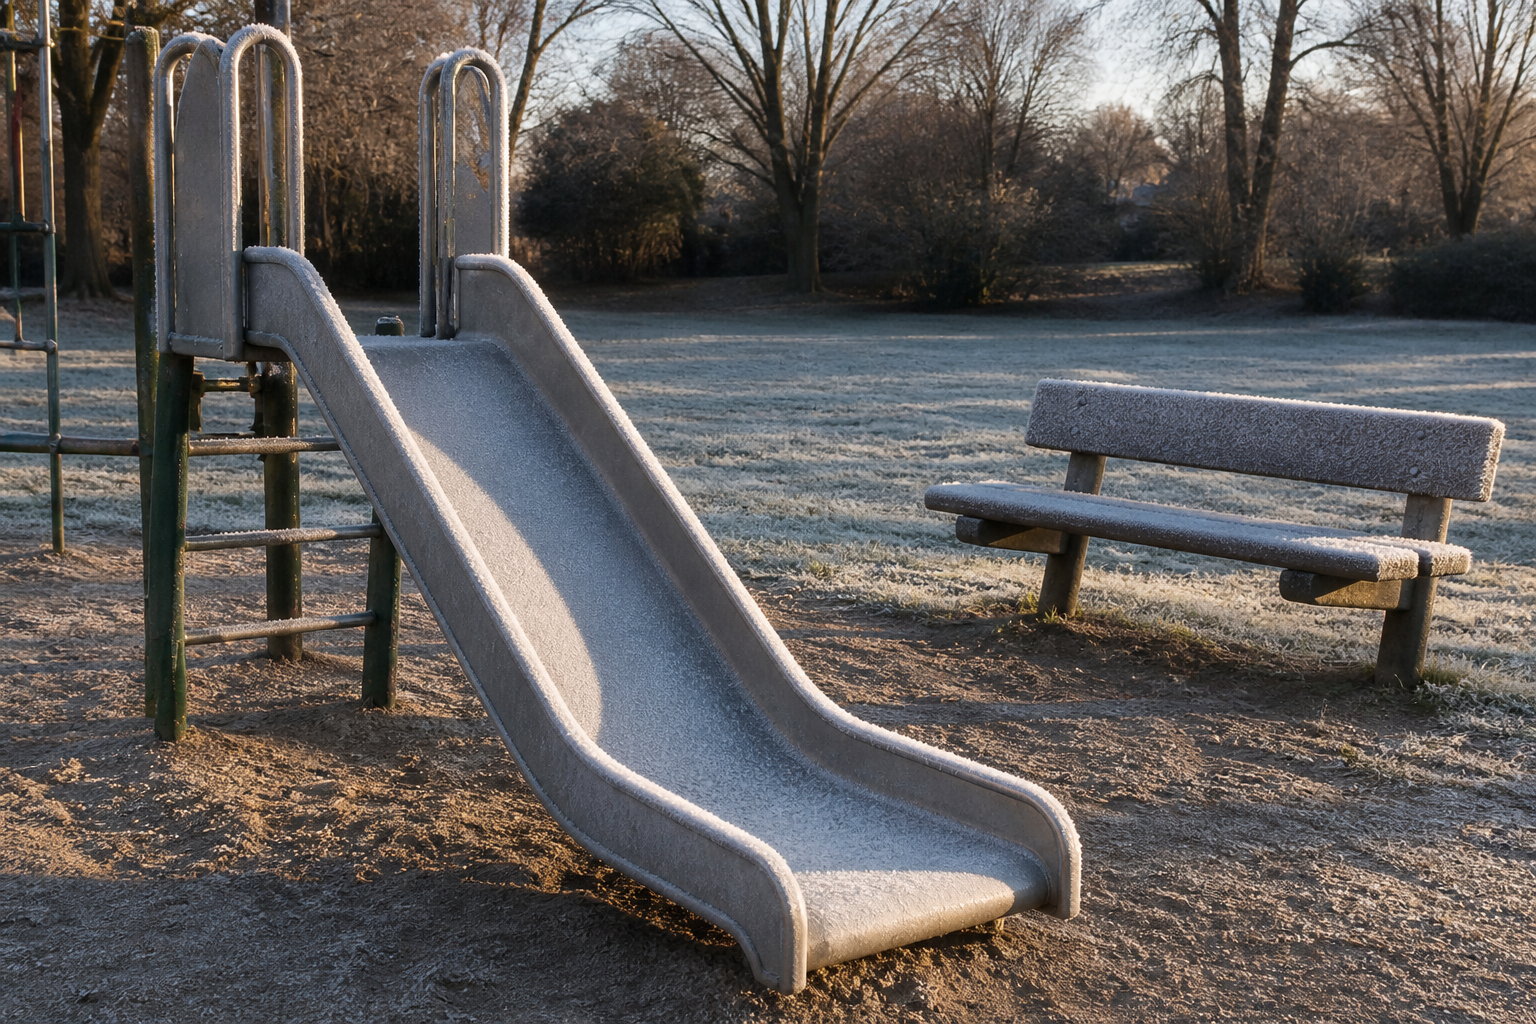
\includegraphics[width=0.58\linewidth]{images/book1/ai/g5-heat-frosty-slide.png}

{\small Uma manhã de geada no parquinho: o escorregador de metal e o banco de madeira passaram a mesma noite na mesma \omterm{def:g3:temperature-thermometers:temperature}{temperatura} --- e mesmo assim só um deles vai morder a sua pele.}
\end{omfigure}

\begin{example}[O mistério do escorregador, resolvido]\label{ex:g5:heat-and-insulation:slide}
O escorregador de metal e o banco de madeira passaram a noite na
mesma \omterm{def:g3:temperature-thermometers:temperature}{temperatura} gelada --- o \omterm{def:g3:temperature-thermometers:temperature}{termômetro} jurou isso faz tempo. Toque
nos dois: a sua mão está mais quente que ambos, então o \omterm{def:g5:heat-and-insulation:heat}{calor} flui de
você para cada um deles. Mas o metal é uma pista rápida --- ele leva
embora o seu \omterm{def:g5:heat-and-insulation:heat}{calor} num rompante, e é esse \emph{rompante} que a gente
sente como ``gelado''. A madeira recebe o seu \omterm{def:g5:heat-and-insulation:heat}{calor} só num fio de
água: mal fica fresca. A sua pele nunca esteve medindo \omterm{def:g3:temperature-thermometers:temperature}{temperatura}
--- ela mede a velocidade da própria perda de \omterm{def:g5:heat-and-insulation:heat}{calor}. Caso encerrado,
quatro anos depois.
\end{example}

\begin{method}[A corrida do esfriamento]\label{met:g5:heat-and-insulation:race}
Veja o isolamento vencer, com números:
\begin{enumerate}
  \item encha duas canecas iguais com água da torneira igualmente
        quente (\emph{peça a um adulto água morna para a mão, não
        fervendo});
  \item enrole uma das canecas com bastante cachecol de lã; deixe a
        outra sem nada;
  \item finque um \omterm{def:g3:temperature-thermometers:temperature}{termômetro} em cada uma e anote as duas \omterm{def:g3:temperature-thermometers:temperature}{temperaturas}
        numa tabela a cada cinco minutos, seis vezes;
  \item desenhe os dois registros como duas linhas num mesmo gráfico,
        \omterm{def:g3:temperature-thermometers:temperature}{temperatura} contra tempo.
\end{enumerate}
A linha da caneca sem nada despenca; a linha da caneca enrolada desce
suavemente. Mesmo começo, mesma sala --- a lã transformou a saída do
\omterm{def:g5:heat-and-insulation:heat}{calor} numa pista lenta.
\end{method}

\begin{omfigure}
\begin{tikzpicture}
\begin{axis}[omaxis, width=10.5cm, height=5.6cm,
    xlabel={minutos}, ylabel={temperatura (\unit{\celsius})},
    xtick={0,5,10,15,20,25,30}, ytick={20,30,40,50},
    ymin=15, ymax=55, xmin=-1, xmax=31]
  \addplot[very thick, omDef] coordinates
    {(0,50) (5,46.5) (10,43.5) (15,41) (20,39) (25,37.5) (30,36)};
  \addplot[very thick, omThm] coordinates
    {(0,50) (5,41) (10,34.5) (15,30) (20,27) (25,24.5) (30,23)};
  \node[right, font=\small, omDef] at (axis cs:24,39.5)
    {enrolada em lã};
  \node[right, font=\small, omThm] at (axis cs:19,25.5) {caneca sem nada};
\end{axis}
\end{tikzpicture}

{\small A corrida do esfriamento, desenhada: duas canecas de água a
\qty{50}{\celsius} numa sala a \qty{20}{\celsius}. A lã não consegue
impedir a fuga do \omterm{def:g5:heat-and-insulation:heat}{calor} --- mas a torna lindamente lenta.}
\end{omfigure}

\begin{remark}[O isolamento apenas retarda]\label{rem:g5:heat-and-insulation:onlyslows}
Olhe para onde as duas curvas estão indo: para os
\qty{20}{\celsius} da sala. Cachecol nenhum, garrafa térmica nenhuma,
parede de iglu nenhuma jamais impede o fluxo do \omterm{def:g5:heat-and-insulation:heat}{calor} ladeira abaixo
--- o isolamento só deixa a pista lenta mais lenta ainda. É também
por isso que o casaco no boneco de neve (lembra dele?) atrasou o
derretimento sem conseguir salvá-lo: o \omterm{def:g5:heat-and-insulation:heat}{calor} do verão continuou
escorrendo para dentro.
\end{remark}

\section{A arte de prender o ar}

\begin{example}[Engenharia de inverno]\label{ex:g5:heat-and-insulation:air}
Quase toda coisa quentinha que você tem é uma máquina de prender \omterm{def:g2:air-around-us:air}{ar}.
A lã aquece você não pelas fibras em si, mas pelos incontáveis
bolsões de \omterm{def:g2:air-around-us:air}{ar} entre elas; os edredons de pena, o fleece e o pardal
inflado feito bolinha num fio congelado jogam todos a mesma carta. As
casas entram na brincadeira: as janelas duplas aprisionam uma camada
de \omterm{def:g2:air-around-us:air}{ar} entre dois vidros, e as paredes isoladas são recheadas com um
enchimento fofo que guarda \omterm{def:g2:air-around-us:air}{ar}. O \omterm{def:g2:air-around-us:air}{ar} parado é a pista lenta campeã ---
o truque é mantê-lo \emph{parado}.
\end{example}

\begin{example}[A garrafa térmica]\label{ex:g5:heat-and-insulation:thermos}
A garrafa térmica é a obra-prima do isolamento: uma garrafa dentro de
outra, com o \omterm{def:g2:air-around-us:air}{ar} entre elas bombeado para fora até quase nada --- e,
onde quase não há material, o fluxo de \omterm{def:g5:heat-and-insulation:heat}{calor} quase não encontra pista
(um truque que vale lembrar: é o mesmo vazio que silenciou a
campainha no frasco). Acrescente paredes espelhadas para devolver o
brilho do \omterm{def:g5:heat-and-insulation:heat}{calor} para dentro, e o chocolate quente encontra a tarde
ainda quente --- ou a limonada ainda gelada: a garrafa térmica não
sabe nada de quente nem de frio, ela só fecha as pistas, nos dois
sentidos.
\end{example}

\begin{remark}[Manter o calor, dito direito]\label{rem:g5:heat-and-insulation:coat}
Agora a velha pergunta do casaco se encerra de vez. Um casaco é \omterm{def:g2:air-around-us:air}{ar}
preso em volta de um fabricante de \omterm{def:g5:heat-and-insulation:heat}{calor} --- você. O seu corpo
despeja \omterm{def:g5:heat-and-insulation:heat}{calor} para fora o dia inteiro; o casaco transforma esse jorro
num fio de água, e você fica quentinho com a sua própria produção. No
boneco de neve --- sem fabricante de \omterm{def:g5:heat-and-insulation:heat}{calor} por dentro --- o mesmo
casaco só retarda o fio de água do verão entrando. O isolamento não
tem preferidos: ele retarda o fluxo, em qualquer sentido que ele
corra.
\end{remark}

\section{Exercícios}

\begin{exercise}[$\star$]\label{exo:g5:heat-and-insulation:1}
O que é \omterm{def:g5:heat-and-insulation:heat}{calor}, e em que sentido ele flui sozinho? Quando o fluxo
para?
\end{exercise}

\begin{exercise}[$\star$]\label{exo:g5:heat-and-insulation:2}
``Feche a porta, você está deixando o frio entrar!'' Reescreva a
frase da avó do jeito que um livro de física escreveria.
\end{exercise}

\begin{exercise}[$\star$]\label{exo:g5:heat-and-insulation:3}
Separe em pistas rápidas e pistas lentas para o \omterm{def:g5:heat-and-insulation:heat}{calor}: uma panela de
cobre; \ um cachecol de lã; \ uma colher de aço; \ \omterm{def:g2:air-around-us:air}{ar} parado; \ uma
colher de pau; \ um edredom.
\end{exercise}

\begin{exercise}[$\star$]\label{exo:g5:heat-and-insulation:4}
Por que as panelas têm fundo de metal mas cabo de plástico ou de
madeira? Responda com as pistas.
\end{exercise}

\begin{exercise}[$\star$]\label{exo:g5:heat-and-insulation:5}
Enfim, com as suas palavras: por que o metal parece mais frio que a
madeira estando na mesma \omterm{def:g3:temperature-thermometers:temperature}{temperatura}? O que a pele mede de verdade?
\end{exercise}

\begin{exercise}[$\star$]\label{exo:g5:heat-and-insulation:6}
Na corrida do esfriamento, por que as duas canecas precisam ser
iguais e começar igualmente quentes? Qual diferença única a
experiência está testando?
\end{exercise}

\begin{exercise}[$\star$]\label{exo:g5:heat-and-insulation:7}
Leia o gráfico do esfriamento: que \omterm{def:g3:temperature-thermometers:temperature}{temperatura} cada caneca marca,
mais ou menos, depois de $15$ minutos? Para qual \omterm{def:g3:temperature-thermometers:temperature}{temperatura} as duas
curvas estão indo, e por quê?
\end{exercise}

\begin{exercise}[$\star$]\label{exo:g5:heat-and-insulation:8}
Por que um pardal se infla feito bolinha num fio congelado? Diga três
invenções humanas que jogam a mesma carta.
\end{exercise}

\begin{exercise}[$\star\star$]\label{exo:g5:heat-and-insulation:9}
A mesma garrafa térmica mantém o chocolate quente em julho e a
limonada gelada em janeiro. Explique como um único objeto dá conta
dos dois serviços --- o que a garrafa térmica faz de fato, e com o
quê?
\end{exercise}

\begin{exercise}[$\star\star$]\label{exo:g5:heat-and-insulation:10}
Uma sorveteira enrola os potes dela em cobertores grossos de lã num
dia quente, e um freguês ri: ``Lã serve para manter as coisas
quentes!'' Defenda a sorveteira com a
\cref{rem:g5:heat-and-insulation:coat} --- em que sentido o \omterm{def:g5:heat-and-insulation:heat}{calor}
está tentando fluir, e o que a lã faz com ele?
\end{exercise}

\begin{exercise}[$\star\star$]\label{exo:g5:heat-and-insulation:11}
Duas casas passam pelo mesmo inverno: uma com janelas simples, outra
com janelas duplas. Explique com as pistas e o \omterm{def:g2:air-around-us:air}{ar} preso por que a
casa de janelas duplas queima menos combustível --- e por que, pela
\cref{rem:g5:heat-and-insulation:onlyslows}, ela ainda precisa de
\emph{algum} aquecimento.
\end{exercise}
